\section{Star Partition and Mining}
\label{sec:spm}
To resolve the two limitations of TRM, we 
propose the \emph{Star Partition and Mining} (SPM) method.
Instead of partition trajectory database in the temporal domain,
SPM partition the trajectory database in the object domain.
Specifically, we design a graph model, named \emph{connection graph}, to capture 
the co-moving behavior among objects. In such a way, 
given an object $u$, all the objects potentially
co-moved with $u$ are captured in $u$'s neighborhood, which
forms a \emph{star} structure in graph terms. SPM utilizes
such structures to partition objects and then adapts an Apriori 
algorithm to discover true GCMPs from each partition.

The flow of SPM method is presented in Figure~\ref{fig:star_partition}.
SPM utilizes the same preprocessing as TRM, thus the flow starts
from clusters in each snapshot. Conceptually, the clusters 
in each snapshot forms a graph as shown in Figure~\ref{fig:star_partition} (a).
In the map phase of \emph{SPM}, a vertex together with its neighborhood 
vertexes form a star. Every star is indeed an independent partition.
Then, stars are shuffled to reducers. As in
Figure~\ref{fig:star_partition} (c), Apriori mining algorithm is adapted
to mine the GCMP patterns. The overview implementation of SPM is shown 
in Algorithm~\ref{algo:spm_overview}.

%The overview of the SPM method is presented in 
%Algorithm~\ref{algo:spm_overview}. As shown, SPM takes three phases. 
%In the map phase, objects from the same cluster form object-object pairs. 
%The object-object pairs are then paired up with the timestamp of 
%the snapshot to form a triplet(lines~\ref{code:spm-map-start}-\ref{code:spm-map-end}). 
%In the partition phase, triplets with the same leading object form a \emph{star} which will be explained shortly 
%(lines~\ref{code:spm-shuffle-start}-\ref{code:spm-shuffle-end}).
%Lastly in the reduce phase, patterns are mined from each star structure (lines~\ref{code:spm-reduce-start}-\ref{code:spm-reduce-end}).

\begin{algorithm}
\caption{Star Partition and Mining}
\label{algo:spm_overview}
\begin{algorithmic}[1]
\Require list of $\langle t, S_t \rangle$ pairs
\State {---Map phase---}
\label{code:spm-map-start}
\ForAll{$C \in S_t$}
	\ForAll {$(o_1 ,o_2) \in C \times C$}
		\If{$o_1 < o_2$}  \label{code:spm-edge-direct}
			\State emit a $\langle o_1, o_2, \{t\}\rangle$ triplet
		\EndIf
	\EndFor
\EndFor
\label{code:spm-map-end}

\State {---Partition and Shuffle phase---}
\label{code:spm-shuffle-start}
\ForAll{$\langle o_1, o_2, \{t\}\rangle$ triplets} 
	\State group-by $o_1$, emit $\langle o_1, Sr_{o_1} \rangle$ 
	%\State group-by $o_2$, emit $\langle o_2, Sr_{o_2} \rangle$
\EndFor
\label{code:spm-shuffle-end}

\State {---Reduce phase---}
\label{code:spm-reduce-start}
\ForAll{$\langle o, Sr_{o} \rangle$}
\State Apriori($Sr_o$)
\EndFor
\label{code:spm-reduce-end}

\end{algorithmic}
\end{algorithm}

\subsection{Star Partition}
The intuition of the star partition is that, if two objects are part 
of the same pattern, they must belong to the same cluster at 
those snapshots. Therefore, we may link objects that belong to 
the same cluster to form the \emph{connection graph}. Objects that are
not connected surely fail to form a pattern. We may then
partition the connection graph based on vertex connectivity
such that mining GCMPs can be done in parallel. 
We formally define the \emph{connection graph} as follows:
\begin{definition}[Connection Graph]
A connection graph is an undirected graph $G=(V:E)$, where 
each $v \in V$ represents an object. An edge $e(s,t)= ET \in E$ 
contains the timestamp sequence at which $s,t$ are in the same cluster,
i.e., $\forall t \in ET, C_t(s) = C_t(t)$. 
\end{definition}

In graph theory, a \emph{star} of a vertex $u$ is the
the set of neighborhood vertexes of $u$. To utilize \emph{star}
partition, since a vertex may appear in multiple stars, 
some replications of vertexes are required. In order to avoid replication 
of edges, we use the \emph{directed star} as follows:

\begin{definition}[Directed Star]
Assign each vertex in $G$ an ID, a direct star of a vertex $s$, denoted as $Sr_s$, 
is the set of incidental edges on $s$
such that $\forall e(s,t) \in Sr_s$, $s < t$. We name $s$
as the \emph{central vertex} of $Sr_s$.
\end{definition}

By leveraging the \emph{directed star}, we avoids replicating the edges. 
A \emph{Connection graph} and \emph{star} examples are 
shown in Figure~\ref{fig:star_partition} (a) and (b). In (a), a connection graph is formed
based on the example in Figure~\ref{fig:related_work}.
In (b), 5 stars are presented. It can be figured out that by leveraging directed star, 
no edges are replicated. In implementation,
as show in Algorithm~\ref{algo:spm_overview} line~\ref{code:spm-edge-direct}, the
comparison between vertices/objects are based on the vertex/object IDs.

\begin{figure*}[t]
\centering
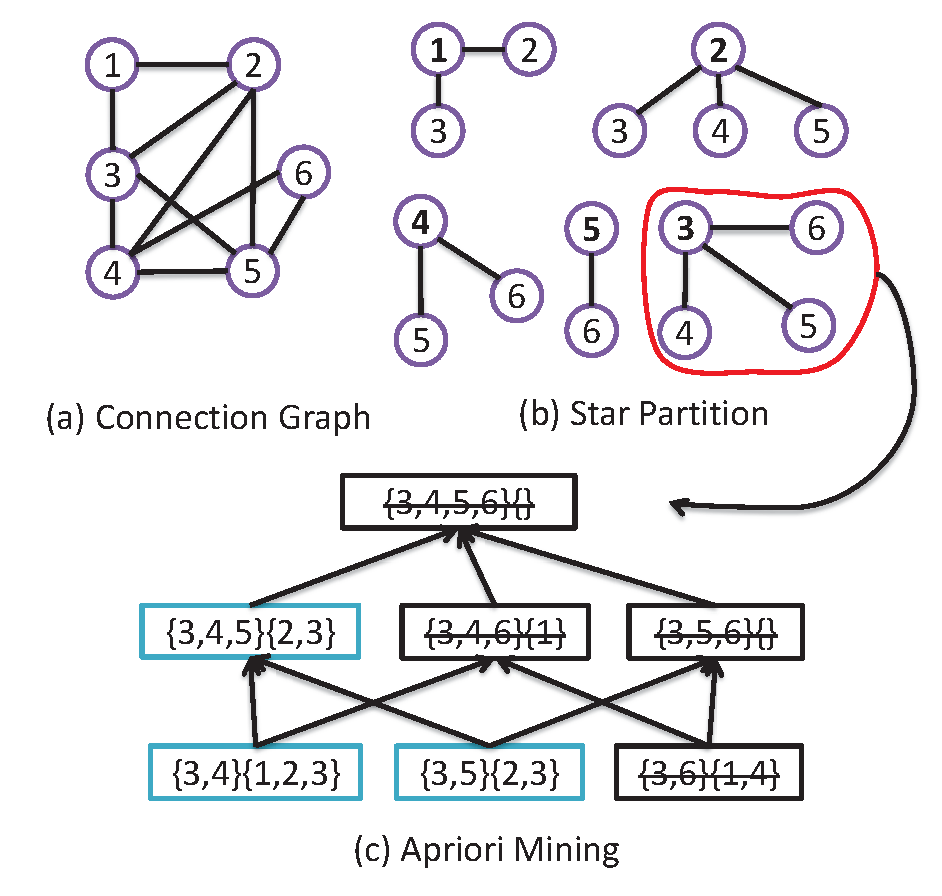
\includegraphics[width=0.9\textwidth]{spm.eps}
\caption{Star partition and mining. (a) Conceptual connection graph from Figure 1.(b) Five star partitions are generated
(c) Apriori Mining with various pruning techniques.}
\label{fig:star_partition}
\end{figure*}

%After computing the star, each partition is applied with a reduce task. 
%Indeed, a star $Sr_s$ can be viewed as a subset of original trajectories. 
%This is done by treating each vertex in $Sr_s$ as an object. 
%The time sequence of $s$ is the union of all edges in $Sr_s$. 
%And the time sequence of $v \neq s$ is the edge $(s,v)$. Therefore, we
%are able to mine stars from the similar trajectory concepts.

\subsection{Apriori Mining}
To systematically discover valid patterns in each star, 
we design the \emph{Apriori Mining} algorithm. 
To describe the  algorithm, we call a candidate pattern $R$-pattern 
if the size of its object set is $R$.  Therefore, each edge
in the star is effectively a $2$-pattern. The intuition of Apriori mining
is the observation that $(R+1)$-patterns can be generated
from $R$-patterns and $2$ patterns. Thus, we may iteratively 
enumerate pattern candidates with all possible sizes.
In particular, initially, for each $e(s,v)=ET$, pattern $p=(\{s,v\}, ET)$ is formed. 
During each iteration, we generate $(R+1)$-patterns by joining $R$-patterns 
with the $2$-patterns. Technically, the join between $p_1=(O_1:T_1)$ and $p_2=(O_2:T_2)$
generates a new pattern $p_3=(O_1 \cup O_2:T_1 \cap T_2)$. Note that in $Sr_s$,
each $R$-pattern contains the object $s$, thus the join only 
grow a $R$-pattern at most to a $(R+1)$-pattern.
Our mining algorithm stops where no further patterns are generated. 
The algorithm is illustrated as in Algorithm~\ref{algo:apriori_mining}.

\begin{algorithm}
\caption{Apriori Mining}
\label{algo:apriori_mining}
\begin{algorithmic}[1]
\Require{$Sr_s$}
\State { Lv $\gets \{\}$,Ground $\gets \{\}$, Output $\gets \{\}$}
\ForAll{$e(s,t) = T \in Sr_s$}
\State{Simply $e(s,t)$} \Comment{Edge Simplification}
\State {Ground.add($\langle \{s,t\}, T \rangle$)}
\State {Lv $\gets$ Ground}
\EndFor
\While{Lv is not empty}
		\State {Lv $\gets$ Lv $\oplus $ Ground}
		\State {Remove false patterns in Lv}
		\Comment{Temporal Monotonicity}
		\If{union of Lv is a valid patter}
			\State{output.add(Lv)} \Comment{Forward Closure}
			\State{break}
		\EndIf
\EndWhile
\State output.addAll($Lv$)
\State \Return output
\end{algorithmic}
\end{algorithm}
 
An illustration of Algorithm~\ref{algo:apriori_mining} is shown in Figure~\ref{fig:star_partition} (c).
As shown, the star $Sr_3=\{3,4,5,6\}$ initially generate three $2$-candidates. At every iteration, 
higher level candidates are generated by joining lower level candidates. When no more candidates 
can be generated, the algorithm stops by outputting the valid patterns.

It is notable that, in star partition, original data is 
replicated at most $O(|\mathbb{O}|)$ times.
In later sections, we will describe several 
more optimization techniques to further reduce the amount of replicated data.
%It is notable that Algorithm~\ref{algo:apriori_mining} takes exponential
%time to mine GCMP. There are two major factors dragging 
%down the performance. First, the size of $Sr_s$ affects the initial 
%size of $2$-patterns. Second, the candidates generated in each 
%level affects the join performance. In later
%sections, we exploit some properties of GCMP to reduce the two factors.

\subsection{Analysis of SPM}
The analysis of SPM contains two parts. We first prove the correctness
of SPM. Then, we analyze the work load distribution of the star sizes.

\subsubsection{Correctness}
An important concern in star partition is that
whether any valid patterns are missed out by 
such a partition. We assert the correctness by 
the following theorem:
\begin{theorem}[Correctness of Star Partition]
\label{THM:SPM_CORRECT}
Star partition is complete.
\end{theorem}

In fact, besides that every valid patterns can be
mined in some stars, star partition further ensures
that patterns discovered
from different star partitions cannot be the same. 
This can be formulated as:

\begin{lemma}[Unique Patterns in Star Partition]
\label{LEM:SPM_CORRECT}
Let $Sr_i$ and $Sr_j$ ($i\neq j$) be two stars. Let $P_i$ (resp. $P_j$) be 
the patterns discovered from $Sr_i$ (resp. $P_j$). 
Then, $\forall p_i \in P_i, \forall p_j \in P_j, p_i.O \not\equiv p_j.O$.
\end{lemma}

This lemma indicates that every star partition discovers different patterns,
thus less redundant work could exist as opposed to the line sweep method in TRM.

\subsubsection{Optimal Star Partition}
An important concern in designing a partition 
algorithm is the skewed execution times for
each partition. If there are partitions
taking significant long time to execute, they would become
the bottleneck of the entire system. Such long time-taken partitions
are referred as \emph{stragglers}~\cite{kwon2012skewtune,xin2013shark,coppa2015data}. In TRPM, where
each partition contains a equal-sized snapshots, the \emph{straggler}
is not a concern. However, in SPM, the size distribution of
stars remains unknown. It is necessary to analyze the 
distribution of SPM workloads. We use $\Gamma$ to indicate
the size of \emph{straggler} in star partition. Intuitively,
a large $\Gamma$ means the system has a more prominent bottleneck. 
And smaller $\Gamma$ is always preferred.

% As we shown in Algorithm~\ref{algo:apriori_mining},
%the running time of a star partition is correlated with the number of edges.
%Therefore, we use the number of edges to measure the \emph{straggler}, where
%the \emph{straggler} refers to the largest star. W.L.O.G, we use $\Gamma$ to
%denote the size of the \emph{straggler}. Intuitively, a large $\Gamma$ indicates
%a large straggler

%
%We use the conventional indicator \emph{straggler} to analyze the distribution of SPM, where 
%the \emph{straggler} is determined by the largest size of stars 
%in the SPM. Intuitively, a large \emph{straggler} 

%An important concern in design 
%the distribution of work loads. 
%Traditionally, the quality of a partition strategy 
%is measured based on two aspects: (1) the number of result partition, which
%affects the maximum parallelism
%(2) the size balance of partitions, which affects the finishing
%time of a job. 
%
%Unlike TRM where each partition
%contains equal-sized snapshots, the size distribution 
%of stars in SPM remains unknown. To formally analyze
%the distribution of SPM workloads, we use the concept 
%of \emph{strangler} 



%Nevertheless, we notice that, in SPM, the total sizes of 
%stars are invariant. Therefore, the quality of a star partition
%can be formalized as the \emph{skewness}, which is the maximum star size
%among all stars. Smaller \emph{skewness} naturally results in more partitions
%and less imbalance.


\begin{figure}[h]
\centering
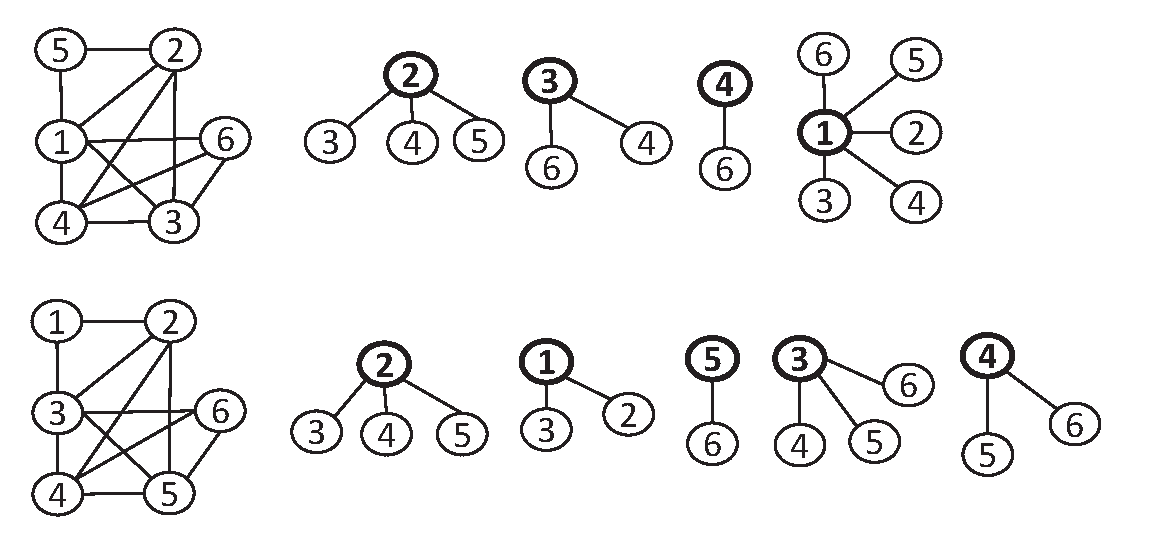
\includegraphics[width=0.5\textwidth]{star-alt.eps}
\caption{An alternative numbering and partitioning of the connection graph in Figure~\ref{fig:star_partition}.}
\label{fig:star-alt}
\end{figure}

Interestingly, we note that the size of \emph{straggler} (i.e., $\Gamma$) 
of star partition is affected by
the way the vertexes are numbered in the aggregate graph. For example,
Figure~\ref{fig:star-alt} gives two valid numbering of vertexes 
of the same aggregate graph, but produces two different set of stars. 
The upper partitioning constructs 4 stars with the maximum star consisting of 5 edges.
The lower partitioning constructs 5 stars with the maximum star consisting of 3 edges.
Apparently the upper partitioning is inferior because its $\Gamma$ is 5 while the
lower one's $\Gamma$ is 3.

Ideally we wish to find a numbering scheme of aggregate graph
that minimize the size of straggler, (i.e, $\Gamma$).
To quantify, we use an linear algebra model as follows: 
Let $G$ be an aggregate graph, with a $n \times n$ adjacent matrix $A$.
A numbering scheme is in fact a permutation of $A$. Therefore,
the adjacent matrix of a numbered graph can be represented as $PAP^T$
where $P \in \mathbb{P}$ is a 
\emph{permutation matrix}~\footnote{an identity matrix with rows shuffled} with dimension $n$.
Since in SPM we assign each edge $e(i,j)$ to the lower vertex, 
then the matrix $B=\text{triu}(PAP^T)$~\footnote{\text{triu} is the upper triangle part of a matrix}
represents the assignment matrix wrt. $P$ (i.e., $b_{i,j} = 1$ if vertex $j$ is in star $Sr_i$).
%Let $P \in \mathbb{P}$ be a \emph{permutation matrix} with dimension $n$.
%Then numbering with $P$ generates an adjacent matrix $B = PAP^T$.
%Let $\mathbb{A}$ be
%the set of all numbering schemes. A numbering scheme
%$A \in \mathbb{A}$ is a boolean assignment matrix 
%(i.e., $a_{i,j} \in A $ indicates whether vertex $j$ is included in $Sr_i$. Apparently, $a_{i,j} \neq a_{j,i}$).
%%Let $\mathbb{A}$ be an arbitrary numbering of vertexes in $G$.
%Given a numbering scheme, let $(A:a_{i,j})$ be a boolean assignment matrix
%(i.e., $a_{i,j}$ indicates whether vertex $j$ is included in $Sr_i$).
Let vector $\vec{b}$ be the \textit{one}\footnote{every element in $\vec{b}$ is $1$} 
vector. Let $\vec{c} = B\vec{b}$, then each $c_i \in \vec{c}$ 
denotes the size of the star $Sr_i$. Thus, $\Gamma$ can be represented
as the infinity norm of $B\vec{b}$. The minimum size of straggle, $\Gamma^*$
can then be formulated as follows:
\begin{equation}
\Gamma^* = \min_{P \in \mathbb{P}}{||B\vec{b}||_\infty} \text{ ,where } ||B\vec{b}||_\infty = \max_{1\leq j \leq n}(c_j)
\end{equation}

It is challenging to directly optimize the above equation. 
First, suppose there are $n!$ permutation matrices. 
Such a high complexity is trivially unpractical. Second,
since $G$ is unknown in prior,
the load planning cannot be done beforehand. 
Despite these challenges, we observe that there is a 
$O(1)$ time solution which is good enough as stated in the 
following theorem.

\begin{theorem}[Balance of Star Partition]
\label{THM:SPM_LB}
Let $G$ be an aggregated graph with $n$ vertexes and the average degree $d$.
Let $\Gamma^*$ be optimal size of straggler.
Let $\Gamma$ be the size of straggler wrt an random numbering $P$. 
With high probability, the difference between $\Gamma$ and $\Gamma^*$ is $O(\sqrt{n \log n})$.
That is,  with probability $1-1/n$, 
$\Gamma = \Gamma^* + O(\sqrt{n \log n})$.
\end{theorem}

In fact, we have a tighter bound of $\Gamma - \Gamma^*$ if 
the aggregate graph is \emph{dense}. Specifically, if $d\geq \sqrt{12\log n}$, with
high probability, $\Gamma = \Gamma^* + O(\sqrt{d\log n})$.
Utilizing Theorem~\label{THM:SPM_LB}, in SPM, it is safe to choose the object IDs as 
the vertex number. This because in reality, object IDs are often 
hashed and can be deemed as random.